\vspace{-3mm}
\section{Evaluation of Uncertainty Quantification in RL}
\label{sec:experiments}

\looseness=-1
In this section, we provide an extensive evaluation of uncertainty estimation for model-free RL. It compares four uncertainty estimation methods for model-free RL in three environments. First, we evaluate the uncertainty predictions at \emph{training time} to assess the uncertainty concentration (des.~\ref{ax:training_state}) and the sample efficiency of the uncertainty-guided exploration-exploitation strategy (des.~\ref{ax:training_strategy}). Second, we evaluate the uncertainty estimates at \emph{testing time} to assess the OOD detection performances (des.~\ref{ax:testing_state}) and the generalization performances of the uncertainty-guided decision strategy (des.~\ref{ax:testing_strategy}). In particular, we evaluate the trade-off between the generalization performance and the detection performance in new perturbed test environments.

\looseness=-1
\textbf{Models.} We consider the four uncertainty models MC Dropout \textbf{(DropOut)}, \textbf{Ensemble}, deep kernel learning \textbf{(DKL)} and the evidential model based on Posterior Networks \textbf{(PostNet)} combined with the DQN RL policy (see sec.~\ref{sec:models}). In this work, we focus on DQN \cite{dqn} since it is a widely used model-free RL agent which does not provide any uncertainty estimates by default. All models use the same encoder architecture and DQN hyper-parameters. We performed a grid search over all hyper-parameters. We compute the mean and standard error of the mean over 5 seeds. Further details are given in app.~\ref{app:models-details}.

\looseness=-1
\textbf{Environments.} We used three training environments \textbf{CartPole} \cite{cartpole}, \textbf{Acrobot} \cite{acrobot1, acrobot2} and \textbf{LunarLander} \cite{lunarlander1, lunarlander2} from the Open AI gym environments \cite{gym}. \citet{assessing-generalization-rl} also used similar environment to assess generalization in RL. We focus on these environments since they turn out to be already challenging settings for the uncertainty methods and the sampling strategies. Some methods and strategies are indeed already unable to achieve high performance for sample efficiency, generalization, and OOD detection. We provide further details on the environments in app.~\ref{app:environments-details}. \textit{\underline{OOD environments:}} The states, actions, and transition dynamics of the OOD environments should not be relevant to the original training environment task, thus being a reasonable failure mode. To this end, the input state is composed of Gaussian noise at every time step independently of the previous actions. \textit{\underline{Perturbed environments:}} These environments are perturbed versions of the original training environment with different perturbation strengths. We separately perturb the \emph{state} space, the \emph{action} space, and the \emph{transition} dynamics with different strengths of Gaussian or uniform noises. These perturbations follow the MDP structure of the environment as proposed by the formal framework for domain shifts presented in \cite{domain-shifts-rl}. We did not consider perturbation on the initial state only, which would be a weaker version of the state perturbations, and perturbations on the reward function which would not affect the model at testing time. Further details are given in app.~\ref{app:environments-details}.

\looseness=-1
\textbf{Training Time.} First, we compare the sample efficiency and the uncertainty predictions of the four uncertainty methods using the epsilon-greedy exploration-exploitation strategy at training time. We normalize the epistemic uncertainty in $[0, 1]$ with min-max normalization to compute the relative epistemic uncertainty. It allows us to easily compare the trend of the epistemic uncertainty of all models. We show the key results for Cartpole in fig.~\ref{fig:model-training-testing-performance-cartpole-main} and the detailed results for CartPole, Acrobot and LunarLander in fig.~\ref{fig:model-training-performance-cartpole}, \ref{fig:model-training-performance-acrobot}, \ref{fig:model-training-performance-lunarlander} in app.~\ref{app:additional-experiments}. We observe that all methods achieve similar sample efficiency. Ensemble with epsilon-greedy strategy struggles to maintain high reward on CartPole. This can be intuitively explained by the under-exploration of the epsilon-greedy strategy as also observed by \citet{randomized-prior-functions, dropout}. Further, we observe that only the epistemic uncertainty estimates of the combination of DQN and PostNet decreases during training. Thus, PostNet \emph{empirically} validates des.~\ref{ax:training_state}. In contrast, the epistemic uncertainty estimates of other methods increase or do not converge. This corroborates with the findings of \cite{randomized-prior-functions} which \emph{theoretically} shows that the uncertainty estimates of dropout and ensemble might not converge even on simple tasks.

\begin{figure*}
    \centering
    \vspace{-5mm}
        \begin{subfigure}{.5\textwidth}
        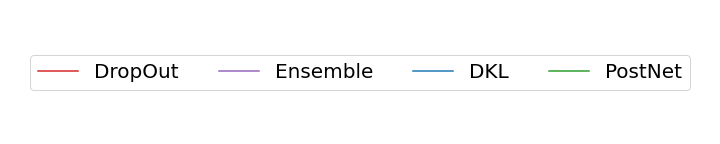
\includegraphics[width=\textwidth]{sections/011_icml2022/resources/legend.png}
    \end{subfigure}
    \vspace{-7mm}
    
    \begin{subfigure}{.23\textwidth}
        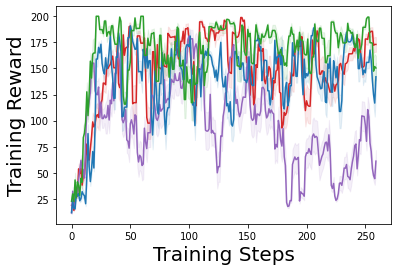
\includegraphics[width=\textwidth]{sections/011_icml2022/resources/cartpole-training_total_reward-training-model.png}
        \vspace{-5mm}
        \caption{}
         \label{fig:model-training-reward-cartpole}
   \end{subfigure}
    \begin{subfigure}{.23\textwidth}
        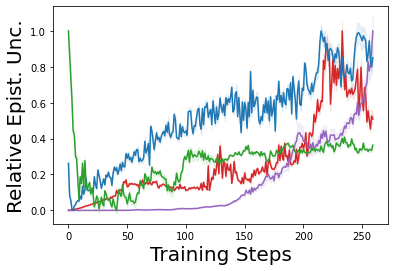
\includegraphics[width=\textwidth]{sections/011_icml2022/resources/cartpole-training_epistemic_uncertainty-training-model.png}
        \vspace{-5mm}
        \caption{}
        \label{fig:model-training-uncertainty-cartpole}
    \end{subfigure}
    \begin{subfigure}{.23\textwidth}
        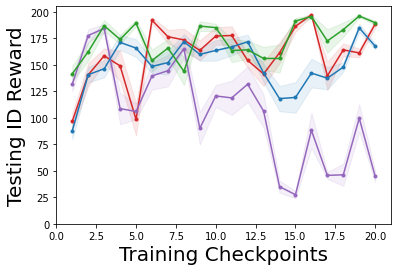
\includegraphics[width=\textwidth]{sections/011_icml2022/resources/CartPole-v0-mean_reward_-testing-model.png}
        \vspace{-5mm}
        \caption{}
        \label{fig:model-testing-reward-cartpole}
    \end{subfigure}
    \begin{subfigure}{.23\textwidth}
        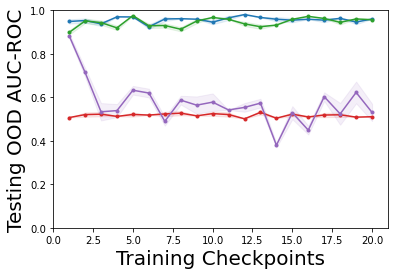
\includegraphics[width=\textwidth]{sections/011_icml2022/resources/CartPoleOOD-v0-AUC-ROC-epistemic_-testing-model.png}
        \vspace{-5mm}
        \caption{}
        \label{fig:model-testing-ood-cartpole}
    \end{subfigure}
    \vspace{-3mm}
    \caption{Comparison of the training performance (\ref{fig:model-training-reward-cartpole},  \ref{fig:model-training-uncertainty-cartpole}) and testing performance (\ref{fig:model-testing-reward-cartpole},  \ref{fig:model-testing-ood-cartpole}) of the four uncertainty methods using epsilon-greedy strategies on CartPole. Ideally, an uncertainty aware-model in RL should achieve high reward with few training samples at training and testing time, a decreasing epistemic uncertainty at training time and high OOD detection scores at testing time.}
    \label{fig:model-training-testing-performance-cartpole-main}
    \vspace{-5mm}
\end{figure*}

\looseness=-1
Second, we compare the sample and episode efficiency of the \emph{sampling-epistemic} and the \emph{sampling-aleatoric} strategies for each model during training. We show the results for Acrobot in fig.~\ref{fig:strategy-training-performance-acrobot-main}, and additional results for CartPole and LunarLander in fig.~\ref{fig:strategy-training-performance-cartpole}, \ref{fig:strategy-training-performance-lunarlander} in app.~\ref{app:additional-experiments}. We observe that all models achieve high rewards by using the sampling-epistemic strategy. In particular, we observed that Ensemble with epistemic sampling achieves more stable rewards than with epsilon-greedy which aligns with observations in \cite{bootstrapped-dqn}. Further, we observe that all models instantiating both aleatoric and epistemic uncertainty achieve significantly better sample efficiency with sampling-epistemic than sampling-aleatoric. Contrary to the sampling-epistemic strategy, the sampling-aleatoric strategy intuitively fails at visiting new under-explored states/actions, thus achieving low and unstable rewards. Hence, Drop-Out, Ensemble and PostNet \emph{empirically} validate des.~\ref{ax:training_strategy}. Thus, disentangling aleatoric and epistemic uncertainty can speed learning in a training environment. Further, the sampling-epistemic strategy requires fewer finished episodes on CartPole and LunarLander. This represents a more reliable training for these two environments since each finished episode translates into a failure and a restart of the systems (see app.~\ref{app:additional-experiments}).

%\begin{figure}
    \centering
    \begin{subfigure}{.45\textwidth}
        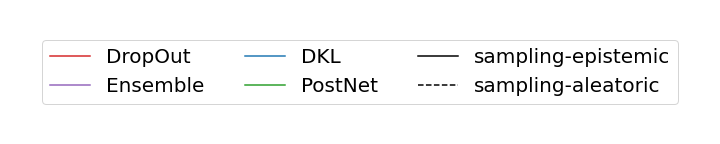
\includegraphics[width=\textwidth]{sections/011_icml2022/resources/sampling-legend.png}
    \end{subfigure}
    \vspace{-3mm}
    
    \begin{subfigure}{.245\textwidth}
        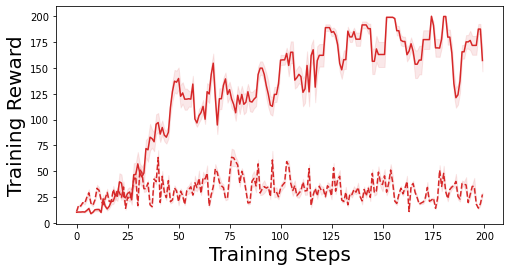
\includegraphics[width=\textwidth]{sections/011_icml2022/resources/cartpole-training_total_reward-dropout-training-strategy.png}
    \end{subfigure}
    \begin{subfigure}{.245\textwidth}
        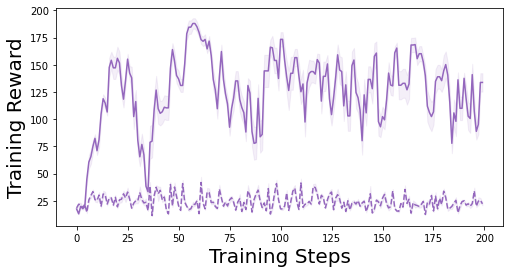
\includegraphics[width=\textwidth]{sections/011_icml2022/resources/cartpole-training_total_reward-ensemble-training-strategy.png}
    \end{subfigure}
    \begin{subfigure}{.245\textwidth}
        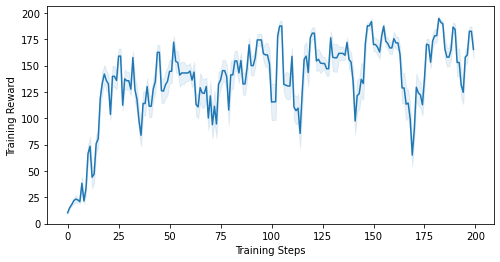
\includegraphics[width=\textwidth]{sections/011_icml2022/resources/cartpole-training_total_reward-dkl-training-strategy.png}
    \end{subfigure}
    \begin{subfigure}{.245\textwidth}
        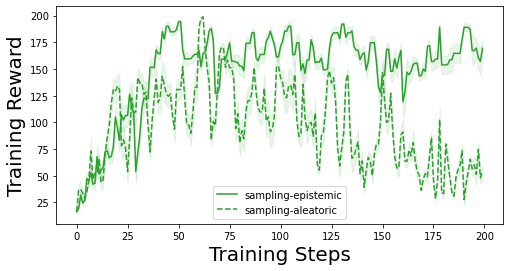
\includegraphics[width=\textwidth]{sections/011_icml2022/resources/cartpole-training_total_reward-postnet-training-strategy.png}
    \end{subfigure}
    
    \begin{subfigure}{.245\textwidth}
        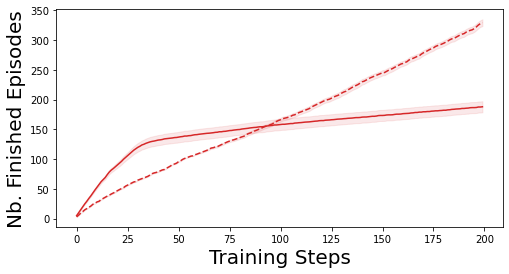
\includegraphics[width=\textwidth]{sections/011_icml2022/resources/cartpole-n_finished_training_episodes-dropout-training-strategy.png}
    \end{subfigure}
    \begin{subfigure}{.245\textwidth}
        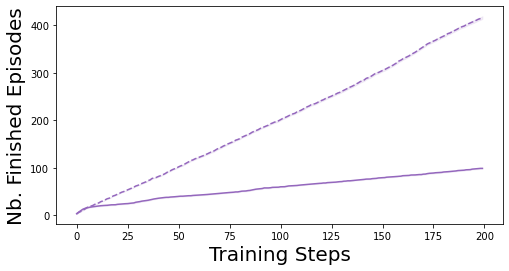
\includegraphics[width=\textwidth]{sections/011_icml2022/resources/cartpole-n_finished_training_episodes-ensemble-training-strategy.png}
    \end{subfigure}
    \begin{subfigure}{.245\textwidth}
        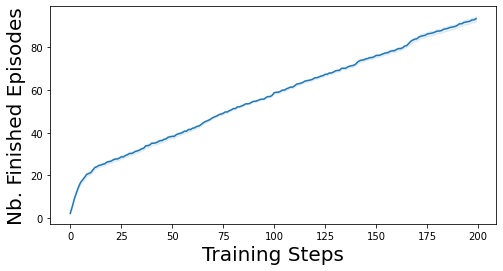
\includegraphics[width=\textwidth]{sections/011_icml2022/resources/cartpole-n_finished_training_episodes-dkl-training-strategy.png}
    \end{subfigure}
    \begin{subfigure}{.245\textwidth}
        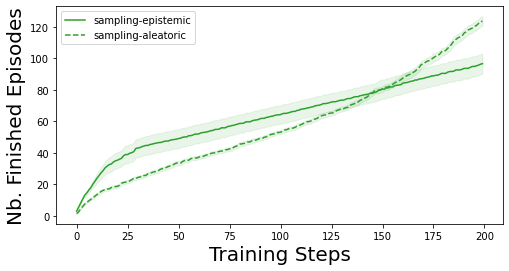
\includegraphics[width=\textwidth]{sections/011_icml2022/resources/cartpole-n_finished_training_episodes-postnet-training-strategy.png}
    \end{subfigure}
    \caption{Comparison of the training performance on Cartpole. The four uncertainty methods use the sampling-aleatoric or the sampling-epistemic at training time. Ideally, an uncertainty aware-model should high reward with few samples.}
    \label{fig:strategy-training-performance-cartpole}
\end{figure}
\begin{figure*}
    \centering
    \vspace{-6mm}
    \begin{subfigure}{.45\textwidth}
        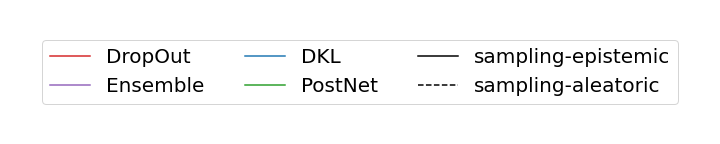
\includegraphics[width=\textwidth]{sections/011_icml2022/resources/sampling-legend.png}
    \end{subfigure}
    \vspace{-4mm}
    
    \begin{subfigure}{.23\textwidth}
        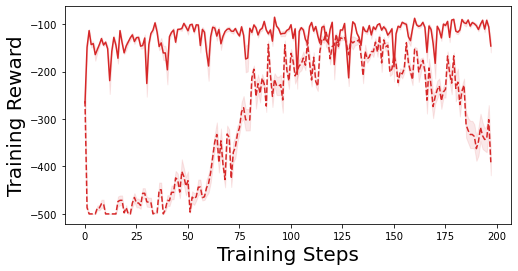
\includegraphics[width=\textwidth]{sections/011_icml2022/resources/acrobot-training_total_reward-dropout-training-strategy.png}
    \end{subfigure}
    \begin{subfigure}{.23\textwidth}
        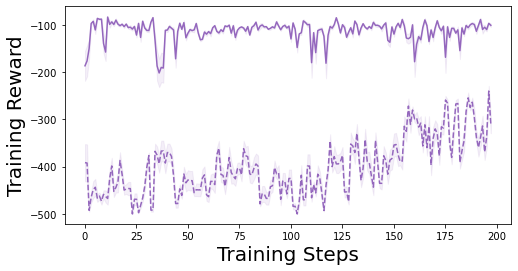
\includegraphics[width=\textwidth]{sections/011_icml2022/resources/acrobot-training_total_reward-ensemble-training-strategy.png}
    \end{subfigure}
    \begin{subfigure}{.23\textwidth}
        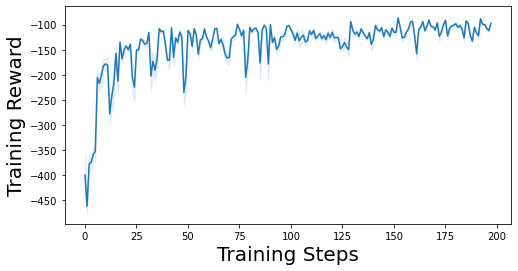
\includegraphics[width=\textwidth]{sections/011_icml2022/resources/acrobot-training_total_reward-dkl-training-strategy.png}
    \end{subfigure}
    \begin{subfigure}{.23\textwidth}
        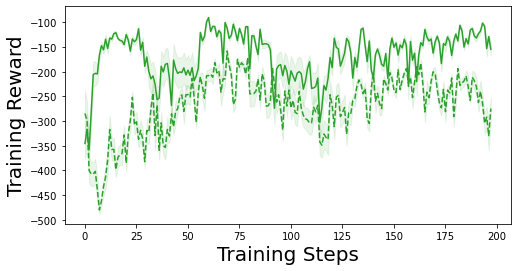
\includegraphics[width=\textwidth]{sections/011_icml2022/resources/acrobot-training_total_reward-postnet-training-strategy.png}
    \end{subfigure}
    
    % \begin{subfigure}{.245\textwidth}
    %     \includegraphics[width=\textwidth]{resources/acrobot-n_finished_training_episodes-dropout-training-strategy.png}
    % \end{subfigure}
    % \begin{subfigure}{.245\textwidth}
    %     \includegraphics[width=\textwidth]{resources/acrobot-n_finished_training_episodes-ensemble-training-strategy.png}
    % \end{subfigure}
    % \begin{subfigure}{.245\textwidth}
    %     \includegraphics[width=\textwidth]{resources/acrobot-n_finished_training_episodes-dkl-training-strategy.png}
    % \end{subfigure}
    % \begin{subfigure}{.245\textwidth}
    %     \includegraphics[width=\textwidth]{resources/acrobot-n_finished_training_episodes-postnet-training-strategy.png}
    % \end{subfigure}
    \vspace{-3mm}
    \caption{Comparison of the training performance on Acrobot. The four uncertainty methods use the sampling-aleatoric or the sampling-epistemic at training time. Ideally, an uncertainty aware-model should high reward with few samples.}
    \label{fig:strategy-training-performance-acrobot-main}
    \vspace{-5mm}
\end{figure*}
% \begin{figure}
    \centering
    \begin{subfigure}{.45\textwidth}
        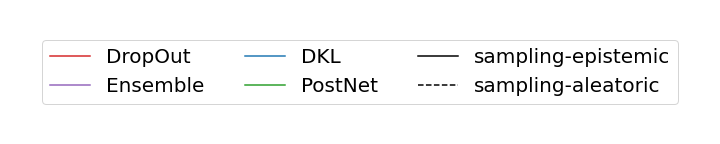
\includegraphics[width=\textwidth]{sections/011_icml2022/resources/sampling-legend.png}
    \end{subfigure}
    \vspace{-3mm}
    
    \begin{subfigure}{.245\textwidth}
        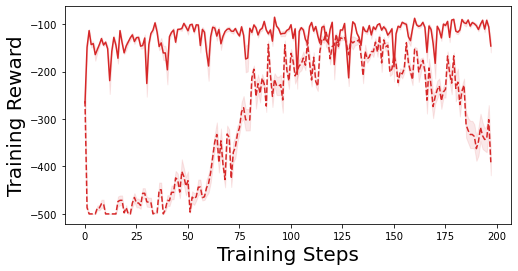
\includegraphics[width=\textwidth]{sections/011_icml2022/resources/acrobot-training_total_reward-dropout-training-strategy.png}
    \end{subfigure}
    \begin{subfigure}{.245\textwidth}
        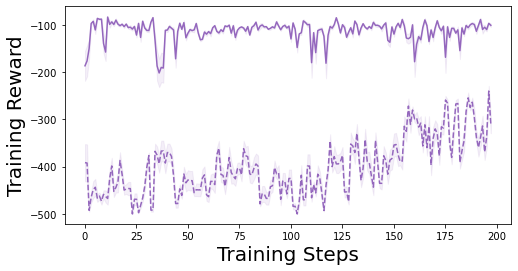
\includegraphics[width=\textwidth]{sections/011_icml2022/resources/acrobot-training_total_reward-ensemble-training-strategy.png}
    \end{subfigure}
    \begin{subfigure}{.245\textwidth}
        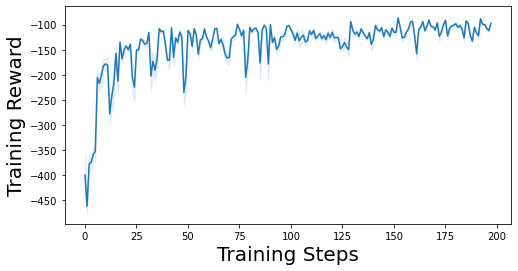
\includegraphics[width=\textwidth]{sections/011_icml2022/resources/acrobot-training_total_reward-dkl-training-strategy.png}
    \end{subfigure}
    \begin{subfigure}{.245\textwidth}
        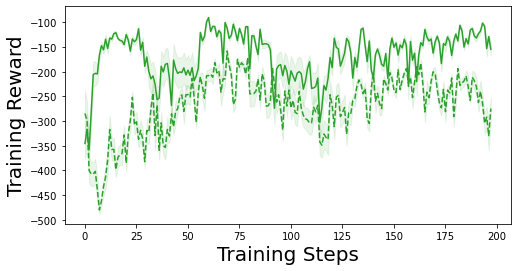
\includegraphics[width=\textwidth]{sections/011_icml2022/resources/acrobot-training_total_reward-postnet-training-strategy.png}
    \end{subfigure}
    
    \begin{subfigure}{.245\textwidth}
        \includegraphics[width=\textwidth]{sections/011_icml2022/resources/acrobot-n_finished_training_episodes-dropout-training-strategy.png}
    \end{subfigure}
    \begin{subfigure}{.245\textwidth}
        \includegraphics[width=\textwidth]{sections/011_icml2022/resources/acrobot-n_finished_training_episodes-ensemble-training-strategy.png}
    \end{subfigure}
    \begin{subfigure}{.245\textwidth}
        \includegraphics[width=\textwidth]{sections/011_icml2022/resources/acrobot-n_finished_training_episodes-dkl-training-strategy.png}
    \end{subfigure}
    \begin{subfigure}{.245\textwidth}
        \includegraphics[width=\textwidth]{sections/011_icml2022/resources/acrobot-n_finished_training_episodes-postnet-training-strategy.png}
    \end{subfigure}
    \caption{Comparison of the training performance on Acrobot. The four uncertainty methods use the sampling-aleatoric or the sampling-epistemic at training time. Ideally, an uncertainty aware-model should high reward with few samples.}
    \label{fig:strategy-training-performance-acrobot}
\end{figure}
%\begin{figure}
    \centering
    \begin{subfigure}{.45\textwidth}
        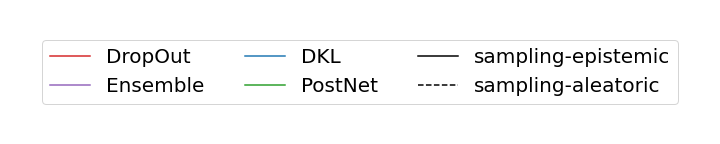
\includegraphics[width=\textwidth]{sections/011_icml2022/resources/sampling-legend.png}
    \end{subfigure}
    \vspace{-3mm}
    
    \begin{subfigure}{.245\textwidth}
        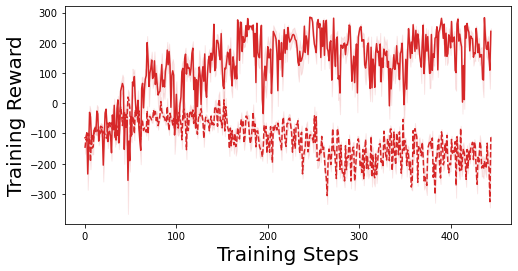
\includegraphics[width=\textwidth]{sections/011_icml2022/resources/lunarlander-training_total_reward-dropout-training-strategy.png}
    \end{subfigure}
    \begin{subfigure}{.245\textwidth}
        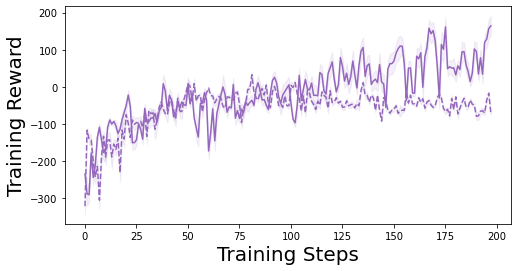
\includegraphics[width=\textwidth]{sections/011_icml2022/resources/lunarlander-training_total_reward-ensemble-training-strategy.png}
    \end{subfigure}
    \begin{subfigure}{.245\textwidth}
        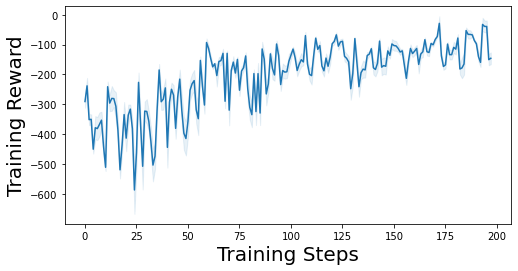
\includegraphics[width=\textwidth]{sections/011_icml2022/resources/lunarlander-training_total_reward-dkl-training-strategy.png}
    \end{subfigure}
    \begin{subfigure}{.245\textwidth}
        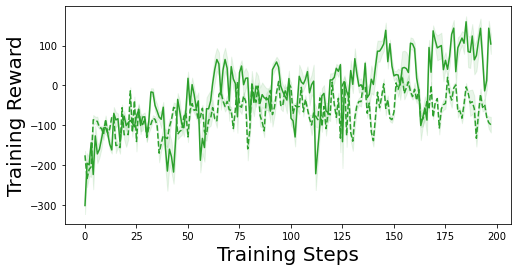
\includegraphics[width=\textwidth]{sections/011_icml2022/resources/lunarlander-training_total_reward-postnet-training-strategy.png}
    \end{subfigure}
    
    \begin{subfigure}{.245\textwidth}
        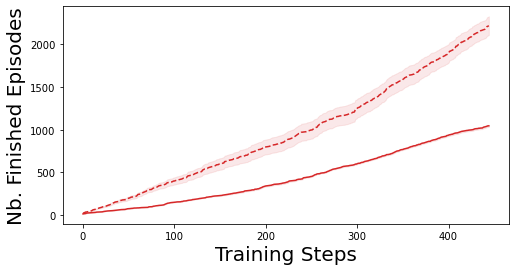
\includegraphics[width=\textwidth]{sections/011_icml2022/resources/lunarlander-n_finished_training_episodes-dropout-training-strategy.png}
    \end{subfigure}
    \begin{subfigure}{.245\textwidth}
        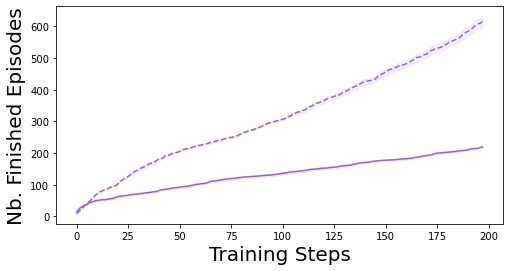
\includegraphics[width=\textwidth]{sections/011_icml2022/resources/lunarlander-n_finished_training_episodes-ensemble-training-strategy.png}
    \end{subfigure}
    \begin{subfigure}{.245\textwidth}
        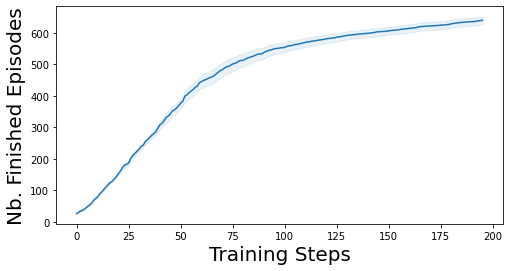
\includegraphics[width=\textwidth]{sections/011_icml2022/resources/lunarlander-n_finished_training_episodes-dkl-training-strategy.png}
    \end{subfigure}
    \begin{subfigure}{.245\textwidth}
        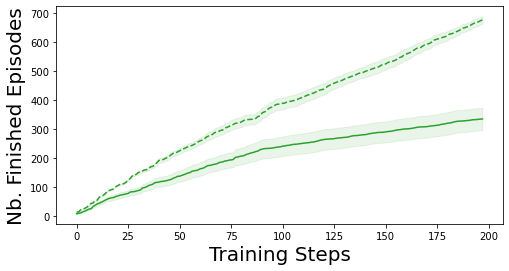
\includegraphics[width=\textwidth]{sections/011_icml2022/resources/lunarlander-n_finished_training_episodes-postnet-training-strategy.png}
    \end{subfigure}
    \caption{Comparison of the training performance on LunarLander. The four uncertainty methods use the sampling-aleatoric or the sampling-epistemic at training time. Ideally, an uncertainty aware-model should high reward with few samples.}
    \label{fig:strategy-training-performance-lunarlander}
\end{figure}

%%% Testing time

\looseness=-1
\textbf{Testing Time.} In this section, we save $20$ models during training to evaluate their performance at testing time. The testing performance can be viewed as the model performance after deployment. First, we evaluate the testing in-distribution (ID) reward in the training environment and the out-of-distribution (OOD) detection performance against the OOD environment composed of fully noisy states. All the methods used the same epsilon-greedy strategy at training time and the action lead to the highest predicted expected return at testing time. The OOD detection performance is measured by comparing the predicted epistemic uncertainty of the states/actions of $10$ episodes with the area under the receiver operating characteristic curve (AUC-ROC). We show the results for CartPole in fig.~\ref{fig:model-training-testing-performance-cartpole-main}, and additional results for Acrobot and LunarLander in fig.~\ref{fig:model-testing-performance-acrobot} and fig.~\ref{fig:model-testing-performance-lunarlander} in app.~\ref{app:additional-experiments}. We observe that DKL and PostNet achieve very high OOD detection scores compared to DropOut and Ensemble. These \emph{empirical} results align with the \emph{theoretical} results stating that DKL and PostNet should assign high uncertainty to states very different from states observed during training. Thus, DKL and PostNet validate des.~\ref{ax:testing_state}. In particular, DKL and PostNet can reliably equip DQN with epistemic uncertainty estimates which can be used to flag anomalous OOD states. In contrast, DropOut and Ensemble achieve poor OOD detection scores. This aligns with \citet{randomized-prior-functions, natpn} which shows on multiple experiments that the uncertainty estimates assigned to OOD inputs by DropOut and Ensemble are not significantly smaller than the uncertainty estimates assigned to inputs close to training data.

%\begin{figure}
    \centering
    \vspace{-7mm}
        \begin{subfigure}{.5\textwidth}
        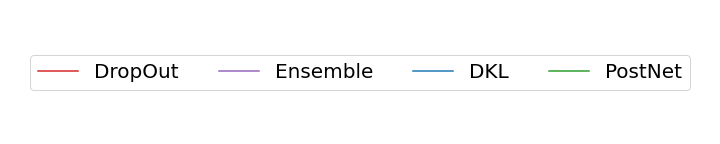
\includegraphics[width=\textwidth]{sections/011_icml2022/resources/legend.png}
    \end{subfigure}
    \vspace{-5mm}
    
    \begin{subfigure}{.4\textwidth}
        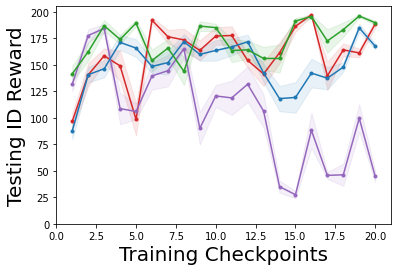
\includegraphics[width=\textwidth]{sections/011_icml2022/resources/CartPole-v0-mean_reward_-testing-model.png}  
    \end{subfigure}
    \begin{subfigure}{.4\textwidth}
        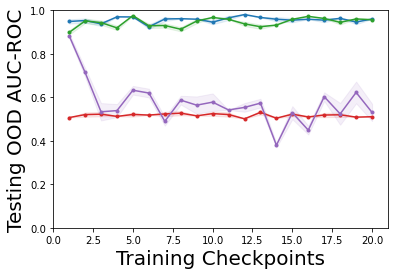
\includegraphics[width=\textwidth]{sections/011_icml2022/resources/CartPoleOOD-v0-AUC-ROC-epistemic_-testing-model.png}
    \end{subfigure}
        \vspace{-3mm}
    \caption{Comparison of the testing performance of the four uncertainty methods using epsilon-greedy strategies at training and testing time on CartPole. Ideally, an uncertainty aware-model should achieve high reward and high OOD detection scores.}
    \label{fig:model-testing-performance-cartpole}
    \vspace{-4mm}
\end{figure}
%\begin{figure}
    \centering
        \begin{subfigure}{.5\textwidth}
        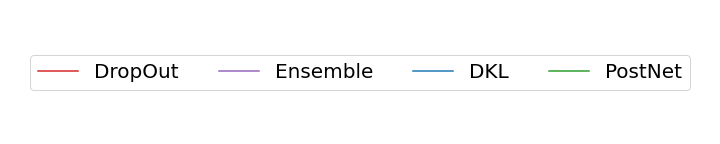
\includegraphics[width=\textwidth]{sections/011_icml2022/resources/legend.png}
    \end{subfigure}
    \vspace{-5mm}
    
    \begin{subfigure}{.4\textwidth}
        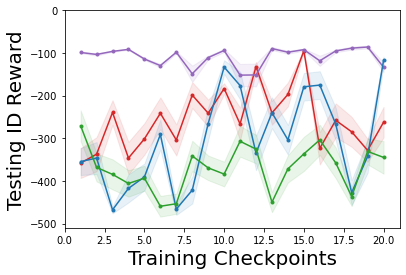
\includegraphics[width=\textwidth]{sections/011_icml2022/resources/Acrobot-v1-mean_reward_-testing-model.png}  
    \end{subfigure}
    \begin{subfigure}{.4\textwidth}
        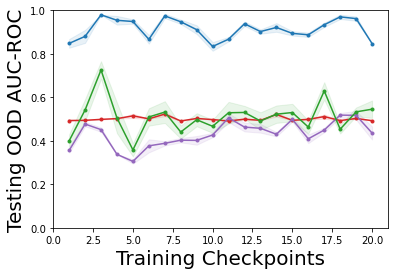
\includegraphics[width=\textwidth]{sections/011_icml2022/resources/AcrobotOOD-v0-AUC-ROC-epistemic_-testing-model.png}
    \end{subfigure}
    \caption{Comparison of the testing performance of the four uncertainty methods using epsilon-greedy strategies at training and testing time on Acrobot. Ideally, an uncertainty aware-model should achieve high reward and high OOD detection scores.}
    \label{fig:model-testing-performance-acrobot}
\end{figure}
%\begin{figure}
    \centering
        \begin{subfigure}{.5\textwidth}
        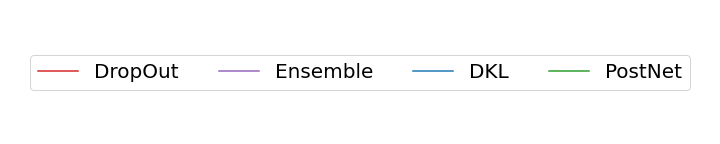
\includegraphics[width=\textwidth]{sections/011_icml2022/resources/legend.png}
    \end{subfigure}
    \vspace{-5mm}
    
    \begin{subfigure}{.4\textwidth}
        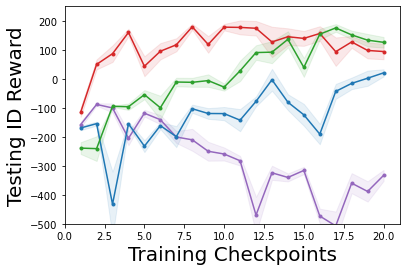
\includegraphics[width=\textwidth]{sections/011_icml2022/resources/LunarLander-v2-mean_reward_-testing-model.png}  
    \end{subfigure}
    \begin{subfigure}{.4\textwidth}
        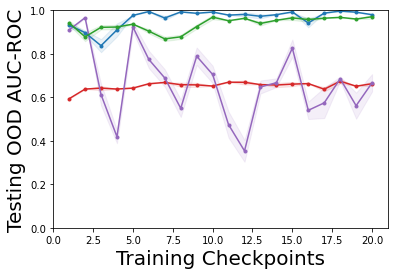
\includegraphics[width=\textwidth]{sections/011_icml2022/resources/LunarLanderOOD-v0-AUC-ROC-epistemic_-testing-model.png}
    \end{subfigure}
    \caption{Comparison of the testing performance of the four uncertainty methods using epsilon-greedy strategies at training and testing time on LunarLander. Ideally, an uncertainty aware-model should achieve high reward and high OOD detection scores.}
    \label{fig:model-testing-performance-lunarlander}
\end{figure}

\looseness=-1
Second, we compare the testing in-distribution (ID) reward and the out-of-distribution (OOD) detection performance when models use the \emph{sampling-aleatoric} and \emph{sampling-epistemic} strategies at \emph{both} training and testing time. We show the results for the testing reward and the OOD detection scores on the LunarLander in fig.~\ref{fig:strategy-testing-performance-lunarlander}, and additional results on the CartPole and the Acrobot environments in fig.~\ref{fig:strategy-testing-performance-cartpole} and fig.~\ref{fig:strategy-testing-performance-acrobot} in app.~\ref{app:additional-experiments}. We observe that the sampling-epistemic strategy achieves significantly better rewards than the sampling-aleatoric for almost any checkpointed models during training. Thus, all models \emph{empirically} satisfy des.~\ref{ax:testing_state}. These empirical results underline the need to disentangle both aleatoric and epistemic uncertainty for high reward performance at testing time.


%\begin{figure}
    \centering
    \begin{subfigure}{.45\textwidth}
        \includegraphics[width=\textwidth]{sections/011_icml2022/resources/sampling-legend.png}
    \end{subfigure}
    \vspace{-3mm}
    
    \begin{subfigure}{.245\textwidth}
        \includegraphics[width=\textwidth]{sections/011_icml2022/resources/DropOut-CartPole-v0-mean_reward_-testing-strategy.png}
    \end{subfigure}
    \begin{subfigure}{.245\textwidth}
        \includegraphics[width=\textwidth]{sections/011_icml2022/resources/Ensemble-CartPole-v0-mean_reward_-testing-strategy.png}
    \end{subfigure}
    \begin{subfigure}{.245\textwidth}
        \includegraphics[width=\textwidth]{sections/011_icml2022/resources/DKL-CartPole-v0-mean_reward_-testing-strategy.png}
    \end{subfigure}
    \begin{subfigure}{.245\textwidth}
        \includegraphics[width=\textwidth]{sections/011_icml2022/resources/PostNet-CartPole-v0-mean_reward_-testing-strategy.png}
    \end{subfigure}
    
    \begin{subfigure}{.245\textwidth}
        \includegraphics[width=\textwidth]{sections/011_icml2022/resources/DropOut-CartPoleOOD-v0-AUC-ROC-epistemic_-testing-strategy.png}
    \end{subfigure}
    \begin{subfigure}{.245\textwidth}
        \includegraphics[width=\textwidth]{sections/011_icml2022/resources/Ensemble-CartPoleOOD-v0-AUC-ROC-epistemic_-testing-strategy.png}
    \end{subfigure}
    \begin{subfigure}{.245\textwidth}
        \includegraphics[width=\textwidth]{sections/011_icml2022/resources/DKL-CartPoleOOD-v0-AUC-ROC-epistemic_-testing-strategy.png}
    \end{subfigure}
    \begin{subfigure}{.245\textwidth}
        \includegraphics[width=\textwidth]{sections/011_icml2022/resources/PostNet-CartPoleOOD-v0-AUC-ROC-epistemic_-testing-strategy.png}
    \end{subfigure}
    \caption{Comparison of the testing reward and OOD performance on CartPole. The four uncertainty methods use the sampling-aleatoric or sampling-epistemic strategies at both training and testing time. Ideally, an uncertainty aware-model should achieve high testing reward and high OOD AUC-ROC detection score.}
    \label{fig:strategy-testing-performance-cartpole}
\end{figure}
%\begin{figure}
    \centering
    \begin{subfigure}{.45\textwidth}
        \includegraphics[width=\textwidth]{sections/011_icml2022/resources/sampling-legend.png}
    \end{subfigure}
    \vspace{-3mm}
    
    \begin{subfigure}{.245\textwidth}
        \includegraphics[width=\textwidth]{sections/011_icml2022/resources/DropOut-Acrobot-v1-mean_reward_-testing-strategy.png}
    \end{subfigure}
    \begin{subfigure}{.245\textwidth}
        \includegraphics[width=\textwidth]{sections/011_icml2022/resources/Ensemble-Acrobot-v1-mean_reward_-testing-strategy.png}
    \end{subfigure}
    \begin{subfigure}{.245\textwidth}
        \includegraphics[width=\textwidth]{sections/011_icml2022/resources/DKL-Acrobot-v1-mean_reward_-testing-strategy.png}
    \end{subfigure}
    \begin{subfigure}{.245\textwidth}
        \includegraphics[width=\textwidth]{sections/011_icml2022/resources/PostNet-Acrobot-v1-mean_reward_-testing-strategy.png}
    \end{subfigure}
    
    \begin{subfigure}{.245\textwidth}
        \includegraphics[width=\textwidth]{sections/011_icml2022/resources/DropOut-AcrobotOOD-v0-AUC-ROC-epistemic_-testing-strategy.png}
    \end{subfigure}
    \begin{subfigure}{.245\textwidth}
        \includegraphics[width=\textwidth]{sections/011_icml2022/resources/Ensemble-AcrobotOOD-v0-AUC-ROC-epistemic_-testing-strategy.png}
    \end{subfigure}
    \begin{subfigure}{.245\textwidth}
        \includegraphics[width=\textwidth]{sections/011_icml2022/resources/DKL-AcrobotOOD-v0-AUC-ROC-epistemic_-testing-strategy.png}
    \end{subfigure}
    \begin{subfigure}{.245\textwidth}
        \includegraphics[width=\textwidth]{sections/011_icml2022/resources/PostNet-AcrobotOOD-v0-AUC-ROC-epistemic_-testing-strategy.png}
    \end{subfigure}
    \caption{Comparison of the testing reward and OOD performance on Acrobot. The four uncertainty methods use the sampling-aleatoric or sampling-epistemic strategies at both training and testing time. Ideally, an uncertainty aware-model should achieve high testing reward and high OOD AUC-ROC detection score.}
    \label{fig:strategy-testing-performance-acrobot}
\end{figure}
\begin{figure*}
    \centering
        % \vspace{-6mm}
    \begin{subfigure}{.45\textwidth}
        \includegraphics[width=\textwidth]{sections/011_icml2022/resources/sampling-legend.png}
    \end{subfigure}
    \vspace{-5mm}
    
    \begin{subfigure}{.2\textwidth}
        \includegraphics[width=\textwidth]{sections/011_icml2022/resources/DropOut-LunarLander-v2-mean_reward_-testing-strategy.png}
    \end{subfigure}
    \begin{subfigure}{.2\textwidth}
        \includegraphics[width=\textwidth]{sections/011_icml2022/resources/Ensemble-LunarLander-v2-mean_reward_-testing-strategy.png}
    \end{subfigure}
    \begin{subfigure}{.2\textwidth}
        \includegraphics[width=\textwidth]{sections/011_icml2022/resources/DKL-LunarLander-v2-mean_reward_-testing-strategy.png}
    \end{subfigure}
    \begin{subfigure}{.2\textwidth}
        \includegraphics[width=\textwidth]{sections/011_icml2022/resources/PostNet-LunarLander-v2-mean_reward_-testing-strategy.png}
    \end{subfigure}
    
    \begin{subfigure}{.2\textwidth}
        \includegraphics[width=\textwidth]{sections/011_icml2022/resources/DropOut-LunarLanderOOD-v0-AUC-ROC-epistemic_-testing-strategy.png}
    \end{subfigure}
    \begin{subfigure}{.2\textwidth}
        \includegraphics[width=\textwidth]{sections/011_icml2022/resources/Ensemble-LunarLanderOOD-v0-AUC-ROC-epistemic_-testing-strategy.png}
    \end{subfigure}
    \begin{subfigure}{.2\textwidth}
        \includegraphics[width=\textwidth]{sections/011_icml2022/resources/DKL-LunarLanderOOD-v0-AUC-ROC-epistemic_-testing-strategy.png}
    \end{subfigure}
    \begin{subfigure}{.2\textwidth}
        \includegraphics[width=\textwidth]{sections/011_icml2022/resources/PostNet-LunarLanderOOD-v0-AUC-ROC-epistemic_-testing-strategy.png}
    \end{subfigure}
        % \vspace{-3mm}
    \caption{Comparison of the testing reward and OOD performance on LunarLander. The four uncertainty methods use the sampling-aleatoric or sampling-epistemic strategies at both training and testing time. Ideally, an uncertainty aware-model should achieve high testing reward and high OOD AUC-ROC detection score.}
    \label{fig:strategy-testing-performance-lunarlander}
        % \vspace{-6mm}
\end{figure*}

\looseness=-1
Third, we compare the \emph{sampling-epistemic} and the \emph{sampling-aleatoric} strategies for each model at testing time. All models use the same epsilon-greedy strategy at training time. We show the key results for the testing reward and the testing epistemic uncertainty on Cartpole with perturbed states, actions, and transition dynamics
% in fig.~\ref{fig:strategy-state-shift-testing-performance-cartpole}, and detailed results with other perturbations and environments 
in app.~\ref{app:additional-experiments}. We observe that stronger state and action perturbations deteriorate the reward performance of all models. This is reasonable since the input state or the output actions become more different from the training environment with stronger perturbations. Further, while the models were trained using the same epsilon-greedy strategy, we observe that the sampling-epistemic strategy generalizes significantly better to all types of perturbed environments than the sampling-aleatoric strategy. In particular, all models achieve high rewards with epistemic sampling on environments with perturbed transitions. Intuitively, sampling-aleatoric select actions with more inherent risk, while the sampling-epistemic select actions accounting for the knowledge accumulated by the agent in the training environment. The generalization capacity of the sampling-epistemic strategy aligns with \cite{epistemic-pomdp} which recast the problem of generalization in RL as solving an epistemic POMDP. Thus, differentiating between aleatoric and epistemic uncertainty can improve generalization. Finally, we observed that DKL and PostNet consistently assign higher epistemic uncertainty to environments with perturbed states which aligns with their theoretical guarantees on extreme input states. The most challenging perturbations are perturbed actions since none of the models provide guarantees for this perturbation type. Overall, DKL and PostNet reliably assign higher epistemic uncertainty to most of the perturbation types. Therefore, DKL and PostNet performs a good trade-off between generalization and detection of new perturbed environments.

% \begin{figure*}
    \centering
        \vspace{-6mm}
    \begin{subfigure}{.45\textwidth}
        \includegraphics[width=\textwidth]{sections/011_icml2022/resources/sampling-legend.png}
    \end{subfigure}
    \vspace{-3mm}
    
    \begin{subfigure}{.24\textwidth}
        \includegraphics[width=\textwidth]{sections/011_icml2022/resources/state_shift-DropOut-CartPoleShift-v0-mean_reward_.png}
    \end{subfigure}
    \begin{subfigure}{.24\textwidth}
        \includegraphics[width=\textwidth]{sections/011_icml2022/resources/state_shift-Ensemble-CartPoleShift-v0-mean_reward_.png}
    \end{subfigure}
    \begin{subfigure}{.24\textwidth}
        \includegraphics[width=\textwidth]{sections/011_icml2022/resources/state_shift-DKL-CartPoleShift-v0-mean_reward_.png}
    \end{subfigure}
    \begin{subfigure}{.24\textwidth}
        \includegraphics[width=\textwidth]{sections/011_icml2022/resources/state_shift-PostNet-CartPoleShift-v0-mean_reward_.png}
    \end{subfigure}
    
    \begin{subfigure}{.24\textwidth}
        \includegraphics[width=\textwidth]{sections/011_icml2022/resources/state_shift-DropOut-CartPoleShift-v0-mean_epistemic_uncertainty_.png}
    \end{subfigure}
    \begin{subfigure}{.24\textwidth}
        \includegraphics[width=\textwidth]{sections/011_icml2022/resources/state_shift-Ensemble-CartPoleShift-v0-mean_epistemic_uncertainty_.png}
    \end{subfigure}
    \begin{subfigure}{.24\textwidth}
        \includegraphics[width=\textwidth]{sections/011_icml2022/resources/state_shift-DKL-CartPoleShift-v0-mean_epistemic_uncertainty_.png}
    \end{subfigure}
    \begin{subfigure}{.24\textwidth}
        \includegraphics[width=\textwidth]{sections/011_icml2022/resources/state_shift-PostNet-CartPoleShift-v0-mean_epistemic_uncertainty_.png}
    \end{subfigure}
        \vspace{-2mm}
    \caption{Comparison of the testing performance and the epistemic uncertainty predictions on CartPole with perturbed states. The four uncertainty methods use the epsilon-greedy strategy at training time and the sampling-aleatoric or sampling-epistemic strategy at testing time. Ideally, an uncertainty-aware model should maintain high reward while assigning higher epistemic uncertainty on more severe perturbations.}
    \label{fig:strategy-state-shift-testing-performance-cartpole}
        \vspace{-6mm}
\end{figure*}
%\begin{figure}
    \centering
    \begin{subfigure}{.45\textwidth}
        \includegraphics[width=\textwidth]{sections/011_icml2022/resources/sampling-legend.png}
    \end{subfigure}
    \vspace{-3mm}
    
    \begin{subfigure}{.245\textwidth}
        \includegraphics[width=\textwidth]{sections/011_icml2022/resources/action_shift-DropOut-CartPoleShift-v0-mean_reward_.png}
    \end{subfigure}
    \begin{subfigure}{.245\textwidth}
        \includegraphics[width=\textwidth]{sections/011_icml2022/resources/action_shift-Ensemble-CartPoleShift-v0-mean_reward_.png}
    \end{subfigure}
    \begin{subfigure}{.245\textwidth}
        \includegraphics[width=\textwidth]{sections/011_icml2022/resources/action_shift-DKL-CartPoleShift-v0-mean_reward_.png}
    \end{subfigure}
    \begin{subfigure}{.245\textwidth}
        \includegraphics[width=\textwidth]{sections/011_icml2022/resources/action_shift-PostNet-CartPoleShift-v0-mean_reward_.png}
    \end{subfigure}
    
    \begin{subfigure}{.245\textwidth}
        \includegraphics[width=\textwidth]{sections/011_icml2022/resources/action_shift-DropOut-CartPoleShift-v0-mean_epistemic_uncertainty_.png}
    \end{subfigure}
    \begin{subfigure}{.245\textwidth}
        \includegraphics[width=\textwidth]{sections/011_icml2022/resources/action_shift-Ensemble-CartPoleShift-v0-mean_epistemic_uncertainty_.png}
    \end{subfigure}
    \begin{subfigure}{.245\textwidth}
        \includegraphics[width=\textwidth]{sections/011_icml2022/resources/action_shift-DKL-CartPoleShift-v0-mean_epistemic_uncertainty_.png}
    \end{subfigure}
    \begin{subfigure}{.245\textwidth}
        \includegraphics[width=\textwidth]{sections/011_icml2022/resources/action_shift-PostNet-CartPoleShift-v0-mean_epistemic_uncertainty_.png}
    \end{subfigure}
    \caption{Comparison of the testing performance and the epistemic uncertainty predictions on CartPole with perturbed actions. The four uncertainty methods use the epsilon-greedy strategy at training time and the sampling-aleatoric or sampling-epistemic strategy at testing time. Ideally, an uncertainty-aware model should maintain high reward while assigning higher epistemic uncertainty on more severe perturbations.}
    \label{fig:strategy-action-shift-testing-performance-cartpole}
\end{figure}
%\begin{figure}
    \centering
        \vspace{-3mm}
    \begin{subfigure}{.45\textwidth}
        \includegraphics[width=\textwidth]{sections/011_icml2022/resources/sampling-legend.png}
    \end{subfigure}
    \vspace{-3mm}
    
    \begin{subfigure}{.245\textwidth}
        \includegraphics[width=\textwidth]{sections/011_icml2022/resources/transition_shift-DropOut-CartPoleShift-v0-mean_reward_.png}
    \end{subfigure}
    \begin{subfigure}{.245\textwidth}
        \includegraphics[width=\textwidth]{sections/011_icml2022/resources/transition_shift-Ensemble-CartPoleShift-v0-mean_reward_.png}
    \end{subfigure}
    \begin{subfigure}{.245\textwidth}
        \includegraphics[width=\textwidth]{sections/011_icml2022/resources/transition_shift-DKL-CartPoleShift-v0-mean_reward_.png}
    \end{subfigure}
    \begin{subfigure}{.245\textwidth}
        \includegraphics[width=\textwidth]{sections/011_icml2022/resources/transition_shift-PostNet-CartPoleShift-v0-mean_reward_.png}
    \end{subfigure}
    
    \begin{subfigure}{.245\textwidth}
        \includegraphics[width=\textwidth]{sections/011_icml2022/resources/transition_shift-DropOut-CartPoleShift-v0-mean_epistemic_uncertainty_.png}
    \end{subfigure}
    \begin{subfigure}{.245\textwidth}
        \includegraphics[width=\textwidth]{sections/011_icml2022/resources/transition_shift-Ensemble-CartPoleShift-v0-mean_epistemic_uncertainty_.png}
    \end{subfigure}
    \begin{subfigure}{.245\textwidth}
        \includegraphics[width=\textwidth]{sections/011_icml2022/resources/transition_shift-DKL-CartPoleShift-v0-mean_epistemic_uncertainty_.png}
    \end{subfigure}
    \begin{subfigure}{.245\textwidth}
        \includegraphics[width=\textwidth]{sections/011_icml2022/resources/transition_shift-PostNet-CartPoleShift-v0-mean_epistemic_uncertainty_.png}
    \end{subfigure}
        \vspace{-2mm}
    \caption{Comparison of the testing performance and the epistemic uncertainty predictions on CartPole with perturbed transitions. The four uncertainty methods use the epsilon-greedy strategy at training time and the sampling-aleatoric or sampling-epistemic strategy at testing time. Ideally, an uncertainty-aware model should maintain high reward while assigning higher epistemic uncertainty on more severe perturbations.}
    \label{fig:strategy-transition-shift-testing-performance-cartpole}
        \vspace{-3mm}
\end{figure}